\documentclass[11pt]{ctexart}
\usepackage[margin=2cm,a4paper]{geometry}
\usepackage{amsthm, amsfonts, amsmath, amssymb, mathrsfs, newclude, tikz-cd, tikz, ctex, mathtools, stmaryrd, datetime}


%\setmainfont{Caladea}

%% 也可以选用其它字库:
% \setCJKmainfont[%
%   ItalicFont=AR PL KaitiM GB,
%   BoldFont=Noto Sans CJK SC,
% ]{Noto Serif CJK SC}
% \setCJKsansfont{Noto Sans CJK SC}
% \renewcommand{\kaishu}{\CJKfontspec{AR PL KaitiM GB}}



\usepackage[colorlinks = true,
linkcolor = blue,
urlcolor  = blue,
citecolor = blue,
anchorcolor = blue]{hyperref}

% Include the x-color package for color support
\usepackage{xcolor}

% Define a new environment for red comments
\usepackage{verbatim} % Required for the comment environment
\usepackage{environ}

\usepackage{mdframed} % Include mdframed for creating framed environments

\definecolor{pinked}{RGB}{255,231,229} % Define a base color 
% Define a new environment with a background color
\newmdenv[
  backgroundcolor=pinked, % Set the desired background color
  linecolor=white, % Optional: Set the border line color
  linewidth=1pt, % Optional: Set the border line width
  roundcorner=5pt, % Optional: Set rounded corners
  nobreak=true % Optional: Prevent page breaks within the environment
]{pinked}

\theoremstyle{definition}
\newtheorem{qqq}{问题}[section]

\newcommand{\ExternalLink}{%
    \tikz[x=1.2ex, y=1.2ex, baseline=-0.05ex]{% 
        \begin{scope}[x=1ex, y=1ex]
            \clip (-0.1,-0.1) 
                --++ (-0, 1.2) 
                --++ (0.6, 0) 
                --++ (0, -0.6) 
                --++ (0.6, 0) 
                --++ (0, -1);
            \path[draw, 
                line width = 0.5, 
                rounded corners=0.5] 
                (0,0) rectangle (1,1);
        \end{scope}
        \path[draw, line width = 0.5] (0.5, 0.5) 
            -- (1, 1);
        \path[draw, line width = 0.5] (0.6, 1) 
            -- (1, 1) -- (1, 0.6);
        }
    }

\NewEnviron{aaa}{~\\
    \noindent {\textcolor{teal}{\textbf{解答}} \BODY }
}

\NewEnviron{llll}{
    \noindent {~\\$\ExternalLink$ 外部链接 $\,\,\,$ \color{blue}\url{\BODY} }
}

\renewcommand{\proofname}{证明}
\renewcommand\qedsymbol{${\boxed{\substack{\textit{完证}\\\textit{毕明}}}}$}


% Define a custom command for \kuing
\newcommand{\kuing}{\texorpdfstring{$\textstyle{\int_u^c k}=\texttt{kuing}$}{}}



% Change equation numbering to include the section number
\usepackage{cleveref}
\renewcommand{\theequation}{\thesection.\thesubsection.\arabic{equation}}
\numberwithin{equation}{section}


%我可以在这里定义一些简化的命令一图便利
\newcommand{\sspan}{\operatorname{span}}%定义span正体
\newcommand{\op}[1]{\operatorname{#1}}%简化函数表达
\newcommand{\cnm}[2]{\binom{#1}{#2} }%简化组合数命令
\newcommand{\set}[2]{\{ #1 \mid #2\}}%定义集合表示
\newcommand{\FF}{\mathbb{F}}%数域
\newcommand{\RR}{\mathbb{R}}
\newcommand{\CC}{\mathbb{C}}
\newcommand{\QQ}{\mathbb{Q}}


%%注意:  行内公式强制行间形式用"  \limits  ",反之用  "  \nolimits   ";
%%注意:  公式引用编号 :" \label{}  ";   公式显示编号" \tag{}  ":  引用公式"  \eqref{}    "


%截止到这里是我定义的

\usepackage{listings}
% Define listings style
\lstset{
  frame=tb,
  language=TeX,
  aboveskip=3mm,
  belowskip=3mm,
  showstringspaces=false,
  columns=flexible,
  basicstyle={\small\ttfamily},
  numbers=none,
  breaklines=true,
  breakatwhitespace=true,
  tabsize=3
}

\theoremstyle{definition}
\newtheorem*{definition}{定义}
\newtheorem*{proposition}{命题}
\newtheorem*{theorem}{定理}
\newtheorem*{notation}{记号}
\newtheorem*{example}{例子}
\newtheorem*{exercise}{习题}
\theoremstyle{remark}
\newtheorem*{remark}{备注}
\newtheorem*{lemma}{引理}
\newtheorem*{corollary}{推论}



\title{高等代数 (荣誉) I 作业模板}
\author{请输入姓名}

\setcounter{section}{-1}

\setcounter{page}{0}

\setlength\parindent{0pt}

\begin{document}

\maketitle

\section{说明}

可以将作业中遇到的问题标注在此. 如有, 请补充.

\tableofcontents

\newpage

%%%%%%%%%%%%%%%%%%%%%%%%%%%%%%%%%%%%%%%%%%%%%%
%%%%%%%%%%%%%%%%%%%%%%%%%%%%%%%%%%%%%%%%%%%%%%
%%%%%%%%%%%%%%%%%%%%%%%%%%%%%%%%%%%%%%%%%%%%%%
%%%%%%%%%%%%%%%%%%%%%%%%%%%%%%%%%%%%%%%%%%%%%%
%%%%%%%%%%%%%%%%%%%%%%%%%%%%%%%%%%%%%%%%%%%%%%
%%%%%%%%%%%%% 请从此处开始阅读 %%%%%%%%%%%%%%%%

\section{中文写作说明}

\subsection{基本规范}

\begin{qqq}
    如何使用标点符号与空格?
    \begin{aaa}
        有一套自己的规范即可 (因为无国标). 例如, 半角 (英文标点) 写作的基本的标点符号包括:
        \begin{table}[h]
            \begin{tabular}{|c|c|c|c|c|c|c|c|c|c|c|}
                \hline
                句号 & 逗号 & 顿号 & 冒号 & 分号 & 左右引号 & 叹号 & 问号 & 书名号 & 左右括号 & $\cdots $ \\ \hline
                .    & ,    & ,    & :    & ;    & `'       & !    & ?    & 无     & ()       & $\cdots $ \\ \hline
            \end{tabular}
        \end{table}

        以下的示例句子足以应付日常写作.
        \begin{enumerate}
            \item 对任意 $\varepsilon >0$, 都存在 $N\in \mathbb N_+$, 使得对一切 $n >N$ 总有 $|x_n-x_0|< \varepsilon$.
            \item 由于连续函数 $f$ 的定义域 $[a,b]$ 是有界闭集, 从而 $\sup_{x\in [a,b]} f(x)$ 可取到 (依照``连续函数映紧集的像为紧集''这一结论).
            \item 记 $S:=\{x\text{ 是集合 }\mid x\notin x\}$, 往证 $S$ 不是集合: 若 $S\in S$, 则依 $S$ 所满足的性质知 $S\notin S$; 反之, 若 $S\notin S$, 则类似的论证表明 $S\in S$. 证明完毕.
        \end{enumerate}
        \begin{pinked}
            若使用微软输入法, 可在中文输入模式下使用 $\texttt{ctrl + .}$, 以切换标点为半角.
        \end{pinked}
    \end{aaa}
\end{qqq}

\begin{qqq}
    如何添加链接?
    \begin{aaa}
        如有引用, 可使用超链接``\href{https://oc.sjtu.edu.cn/courses/72790/assignments/302404}{第一次作业}'', 或使用
        \begin{llll}
            https://oc.sjtu.edu.cn/courses/72790
        \end{llll}
    \end{aaa}
\end{qqq}

\begin{qqq}
    如何用 $\texttt{tikz}$ 绘制矢量图?
    \begin{aaa}
        推荐使用 \href{https://www.mathcha.io/editor}{\texttt{mathcha.io} 的编辑器}进行绘图. 以\href{https://www.mathcha.io/editor/Gjoo6IZYtkXHB3t5MkKrxFQ6yowKfqkok8PUd8w7O}{此}为示例, 依次进行
        \begin{enumerate}
            \item 选中草稿中的任意一张矢量图, 点击上方 \textsf{Tikz} 按钮;
            \item 复制到剪贴板 (\textsf{Copy To Clipboard}), 在 \LaTeX 中直接插入 \texttt{Tikz} 代码即可.
            \item 运行代码, 例如 % 注意: 代码中的 \upPhi 字体缺失, 需要替换作 \Phi. 假如图过大, 会有蓝色报错 \hbox (??pt too wide). 
                  \begin{center}
                      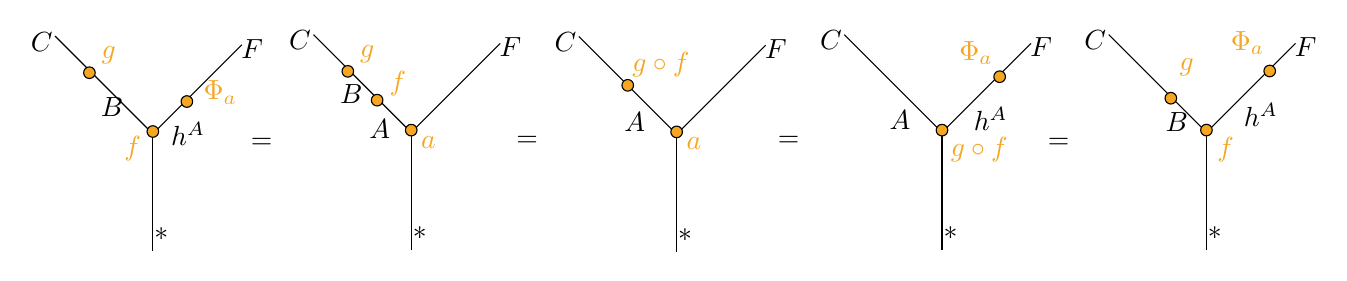
\begin{tikzpicture}[x=0.75pt,y=0.75pt,yscale=-1,xscale=1]
                          %uncomment if require: \path (0,146); %set diagram left start at 0, and has height of 146

                          %Straight Lines [id:da03348217045595492] 
                          \draw    (31.98,15.18) -- (79.08,62.28) ;
                          %Straight Lines [id:da6561022637759857] 
                          \draw    (79.08,62.28) -- (121.98,19.38) ;
                          %Straight Lines [id:da24396426280189765] 
                          \draw    (79.08,62.28) -- (79.08,118.98) ;
                          %Shape: Ellipse [id:dp35145685099177393] 
                          \draw  [fill={rgb, 255:red, 245; green, 166; blue, 35 }  ,fill opacity=1 ] (81.87,61.17) .. controls (81.87,59.63) and (80.62,58.38) .. (79.08,58.38) .. controls (77.54,58.38) and (76.29,59.63) .. (76.29,61.17) .. controls (76.29,62.71) and (77.54,63.96) .. (79.08,63.96) .. controls (80.62,63.96) and (81.87,62.71) .. (81.87,61.17) -- cycle ;
                          %Shape: Ellipse [id:dp0068959474133387655] 
                          \draw  [fill={rgb, 255:red, 245; green, 166; blue, 35 }  ,fill opacity=1 ] (98.27,46.72) .. controls (98.27,45.18) and (97.02,43.93) .. (95.48,43.93) .. controls (93.94,43.93) and (92.69,45.18) .. (92.69,46.72) .. controls (92.69,48.27) and (93.94,49.52) .. (95.48,49.52) .. controls (97.02,49.52) and (98.27,48.27) .. (98.27,46.72) -- cycle ;
                          %Shape: Ellipse [id:dp0688848263542261] 
                          \draw  [fill={rgb, 255:red, 245; green, 166; blue, 35 }  ,fill opacity=1 ] (51.32,32.84) .. controls (51.32,31.29) and (50.07,30.04) .. (48.53,30.04) .. controls (46.98,30.04) and (45.73,31.29) .. (45.73,32.84) .. controls (45.73,34.38) and (46.98,35.63) .. (48.53,35.63) .. controls (50.07,35.63) and (51.32,34.38) .. (51.32,32.84) -- cycle ;
                          %Straight Lines [id:da3117534202393095] 
                          \draw    (156.47,14.52) -- (203.57,61.63) ;
                          %Straight Lines [id:da5228647980485479] 
                          \draw    (203.57,61.63) -- (246.47,18.73) ;
                          %Straight Lines [id:da7379859047826194] 
                          \draw    (203.57,61.63) -- (203.57,118.32) ;
                          %Shape: Ellipse [id:dp4445085865402192] 
                          \draw  [fill={rgb, 255:red, 245; green, 166; blue, 35 }  ,fill opacity=1 ] (206.37,60.52) .. controls (206.37,58.97) and (205.12,57.72) .. (203.57,57.72) .. controls (202.03,57.72) and (200.78,58.97) .. (200.78,60.52) .. controls (200.78,62.06) and (202.03,63.31) .. (203.57,63.31) .. controls (205.12,63.31) and (206.37,62.06) .. (206.37,60.52) -- cycle ;
                          %Shape: Ellipse [id:dp43991467250758043] 
                          \draw  [fill={rgb, 255:red, 245; green, 166; blue, 35 }  ,fill opacity=1 ] (189.93,46.07) .. controls (189.93,44.53) and (188.68,43.27) .. (187.14,43.27) .. controls (185.6,43.27) and (184.35,44.53) .. (184.35,46.07) .. controls (184.35,47.61) and (185.6,48.86) .. (187.14,48.86) .. controls (188.68,48.86) and (189.93,47.61) .. (189.93,46.07) -- cycle ;
                          %Shape: Ellipse [id:dp6572311711882011] 
                          \draw  [fill={rgb, 255:red, 245; green, 166; blue, 35 }  ,fill opacity=1 ] (175.81,32.18) .. controls (175.81,30.64) and (174.56,29.39) .. (173.02,29.39) .. controls (171.48,29.39) and (170.23,30.64) .. (170.23,32.18) .. controls (170.23,33.72) and (171.48,34.97) .. (173.02,34.97) .. controls (174.56,34.97) and (175.81,33.72) .. (175.81,32.18) -- cycle ;
                          %Straight Lines [id:da4637493111853006] 
                          \draw    (284.33,15.36) -- (331.43,62.47) ;
                          %Straight Lines [id:da804684457462356] 
                          \draw    (331.43,62.47) -- (374.33,19.57) ;
                          %Straight Lines [id:da3948927960889712] 
                          \draw    (331.43,62.47) -- (331.43,119.17) ;
                          %Shape: Ellipse [id:dp19631273795974424] 
                          \draw  [fill={rgb, 255:red, 245; green, 166; blue, 35 }  ,fill opacity=1 ] (334.23,61.36) .. controls (334.23,59.81) and (332.98,58.56) .. (331.43,58.56) .. controls (329.89,58.56) and (328.64,59.81) .. (328.64,61.36) .. controls (328.64,62.9) and (329.89,64.15) .. (331.43,64.15) .. controls (332.98,64.15) and (334.23,62.9) .. (334.23,61.36) -- cycle ;
                          %Shape: Ellipse [id:dp5819196420174582] 
                          \draw  [fill={rgb, 255:red, 245; green, 166; blue, 35 }  ,fill opacity=1 ] (310.68,38.92) .. controls (310.68,37.37) and (309.43,36.12) .. (307.88,36.12) .. controls (306.34,36.12) and (305.09,37.37) .. (305.09,38.92) .. controls (305.09,40.46) and (306.34,41.71) .. (307.88,41.71) .. controls (309.43,41.71) and (310.68,40.46) .. (310.68,38.92) -- cycle ;
                          %Straight Lines [id:da5050719128065313] 
                          \draw    (412.19,14.52) -- (459.29,61.63) ;
                          %Straight Lines [id:da18336573583563487] 
                          \draw    (459.29,61.63) -- (502.19,18.73) ;
                          %Straight Lines [id:da4444312893229099] 
                          \draw    (459.29,61.63) -- (459.29,118.32) ;
                          %Shape: Ellipse [id:dp6198851771329514] 
                          \draw  [fill={rgb, 255:red, 245; green, 166; blue, 35 }  ,fill opacity=1 ] (462.09,60.52) .. controls (462.09,58.97) and (460.84,57.72) .. (459.29,57.72) .. controls (457.75,57.72) and (456.5,58.97) .. (456.5,60.52) .. controls (456.5,62.06) and (457.75,63.31) .. (459.29,63.31) .. controls (460.84,63.31) and (462.09,62.06) .. (462.09,60.52) -- cycle ;
                          %Shape: Ellipse [id:dp9406332489043387] 
                          \draw  [fill={rgb, 255:red, 245; green, 166; blue, 35 }  ,fill opacity=1 ] (489.86,34.76) .. controls (489.86,33.21) and (488.61,31.96) .. (487.07,31.96) .. controls (485.52,31.96) and (484.27,33.21) .. (484.27,34.76) .. controls (484.27,36.3) and (485.52,37.55) .. (487.07,37.55) .. controls (488.61,37.55) and (489.86,36.3) .. (489.86,34.76) -- cycle ;
                          %Straight Lines [id:da40223561349822634] 
                          \draw    (539.6,14.49) -- (586.7,61.59) ;
                          %Straight Lines [id:da1407259594634065] 
                          \draw    (586.7,61.59) -- (629.6,18.69) ;
                          %Straight Lines [id:da8441478735262984] 
                          \draw    (586.7,61.59) -- (586.7,118.29) ;
                          %Shape: Ellipse [id:dp7936398048023725] 
                          \draw  [fill={rgb, 255:red, 245; green, 166; blue, 35 }  ,fill opacity=1 ] (589.49,60.48) .. controls (589.49,58.94) and (588.24,57.69) .. (586.7,57.69) .. controls (585.16,57.69) and (583.91,58.94) .. (583.91,60.48) .. controls (583.91,62.03) and (585.16,63.28) .. (586.7,63.28) .. controls (588.24,63.28) and (589.49,62.03) .. (589.49,60.48) -- cycle ;
                          %Shape: Ellipse [id:dp5474614645783034] 
                          \draw  [fill={rgb, 255:red, 245; green, 166; blue, 35 }  ,fill opacity=1 ] (619.98,32.02) .. controls (619.98,30.47) and (618.73,29.22) .. (617.18,29.22) .. controls (615.64,29.22) and (614.39,30.47) .. (614.39,32.02) .. controls (614.39,33.56) and (615.64,34.81) .. (617.18,34.81) .. controls (618.73,34.81) and (619.98,33.56) .. (619.98,32.02) -- cycle ;
                          %Shape: Ellipse [id:dp24424825037675935] 
                          \draw  [fill={rgb, 255:red, 245; green, 166; blue, 35 }  ,fill opacity=1 ] (572.34,45.13) .. controls (572.34,43.59) and (571.08,42.34) .. (569.54,42.34) .. controls (568,42.34) and (566.75,43.59) .. (566.75,45.13) .. controls (566.75,46.67) and (568,47.92) .. (569.54,47.92) .. controls (571.08,47.92) and (572.34,46.67) .. (572.34,45.13) -- cycle ;

                          % Text Node
                          \draw (78.54,106.36) node [anchor=north west][inner sep=0.75pt]    {$\ast $};
                          % Text Node
                          \draw (64.09,61.99) node [anchor=north west][inner sep=0.75pt]  [color={rgb, 255:red, 245; green, 166; blue, 35 }  ,opacity=1 ]  {$f$};
                          % Text Node
                          \draw (19.04,12.09) node [anchor=north west][inner sep=0.75pt]    {$C$};
                          % Text Node
                          \draw (120.41,15.54) node [anchor=north west][inner sep=0.75pt]    {$F$};
                          % Text Node
                          \draw (102.24,35.6) node [anchor=north west][inner sep=0.75pt]  [color={rgb, 255:red, 245; green, 166; blue, 35 }  ,opacity=1 ]  {$\Phi _{a}$};
                          % Text Node
                          \draw (53.14,19.05) node [anchor=north west][inner sep=0.75pt]  [color={rgb, 255:red, 245; green, 166; blue, 35 }  ,opacity=1 ]  {$g$};
                          % Text Node
                          \draw (52.79,43.69) node [anchor=north west][inner sep=0.75pt]    {$B$};
                          % Text Node
                          \draw (86.6,55.4) node [anchor=north west][inner sep=0.75pt]    {$h^{A}$};
                          % Text Node
                          \draw (203.04,105.71) node [anchor=north west][inner sep=0.75pt]    {$\ast $};
                          % Text Node
                          \draw (191.95,31.03) node [anchor=north west][inner sep=0.75pt]  [color={rgb, 255:red, 245; green, 166; blue, 35 }  ,opacity=1 ]  {$f$};
                          % Text Node
                          \draw (143.53,11.44) node [anchor=north west][inner sep=0.75pt]    {$C$};
                          % Text Node
                          \draw (244.9,14.89) node [anchor=north west][inner sep=0.75pt]    {$F$};
                          % Text Node
                          \draw (177.64,18.4) node [anchor=north west][inner sep=0.75pt]  [color={rgb, 255:red, 245; green, 166; blue, 35 }  ,opacity=1 ]  {$g$};
                          % Text Node
                          \draw (168.02,37.14) node [anchor=north west][inner sep=0.75pt]    {$B$};
                          % Text Node
                          \draw (207.1,62.18) node [anchor=north west][inner sep=0.75pt]  [color={rgb, 255:red, 245; green, 166; blue, 35 }  ,opacity=1 ]  {$a$};
                          % Text Node
                          \draw (182.18,53.98) node [anchor=north west][inner sep=0.75pt]    {$A$};
                          % Text Node
                          \draw (330.9,106.55) node [anchor=north west][inner sep=0.75pt]    {$\ast $};
                          % Text Node
                          \draw (308.89,21.77) node [anchor=north west][inner sep=0.75pt]  [color={rgb, 255:red, 245; green, 166; blue, 35 }  ,opacity=1 ]  {$g\circ f$};
                          % Text Node
                          \draw (271.39,12.28) node [anchor=north west][inner sep=0.75pt]    {$C$};
                          % Text Node
                          \draw (372.76,15.73) node [anchor=north west][inner sep=0.75pt]    {$F$};
                          % Text Node
                          \draw (334.96,63.02) node [anchor=north west][inner sep=0.75pt]  [color={rgb, 255:red, 245; green, 166; blue, 35 }  ,opacity=1 ]  {$a$};
                          % Text Node
                          \draw (304.99,50.61) node [anchor=north west][inner sep=0.75pt]    {$A$};
                          % Text Node
                          \draw (458.76,105.71) node [anchor=north west][inner sep=0.75pt]    {$\ast $};
                          % Text Node
                          \draw (399.25,11.44) node [anchor=north west][inner sep=0.75pt]    {$C$};
                          % Text Node
                          \draw (500.62,14.89) node [anchor=north west][inner sep=0.75pt]    {$F$};
                          % Text Node
                          \draw (462.3,62.85) node [anchor=north west][inner sep=0.75pt]  [color={rgb, 255:red, 245; green, 166; blue, 35 }  ,opacity=1 ]  {$g\circ f$};
                          % Text Node
                          \draw (432.85,49.77) node [anchor=north west][inner sep=0.75pt]    {$A$};
                          % Text Node
                          \draw (466.4,16.39) node [anchor=north west][inner sep=0.75pt]  [color={rgb, 255:red, 245; green, 166; blue, 35 }  ,opacity=1 ]  {$\Phi _{a}$};
                          % Text Node
                          \draw (586.16,105.67) node [anchor=north west][inner sep=0.75pt]    {$\ast $};
                          % Text Node
                          \draw (526.66,11.41) node [anchor=north west][inner sep=0.75pt]    {$C$};
                          % Text Node
                          \draw (628.03,14.86) node [anchor=north west][inner sep=0.75pt]    {$F$};
                          % Text Node
                          \draw (590.72,62.82) node [anchor=north west][inner sep=0.75pt]  [color={rgb, 255:red, 245; green, 166; blue, 35 }  ,opacity=1 ]  {$f$};
                          % Text Node
                          \draw (565.77,50.64) node [anchor=north west][inner sep=0.75pt]    {$B$};
                          % Text Node
                          \draw (597.2,11.68) node [anchor=north west][inner sep=0.75pt]  [color={rgb, 255:red, 245; green, 166; blue, 35 }  ,opacity=1 ]  {$\Phi _{a}$};
                          % Text Node
                          \draw (572.52,24.89) node [anchor=north west][inner sep=0.75pt]  [color={rgb, 255:red, 245; green, 166; blue, 35 }  ,opacity=1 ]  {$g$};
                          % Text Node
                          \draw (473.33,48.17) node [anchor=north west][inner sep=0.75pt]    {$h^{A}$};
                          % Text Node
                          \draw (603.45,46.36) node [anchor=north west][inner sep=0.75pt]    {$h^{A}$};
                          % Text Node
                          \draw (124.99,63.07) node [anchor=north west][inner sep=0.75pt]    {$=$};
                          % Text Node
                          \draw (252.99,62.07) node [anchor=north west][inner sep=0.75pt]    {$=$};
                          % Text Node
                          \draw (378.99,62.07) node [anchor=north west][inner sep=0.75pt]    {$=$};
                          % Text Node
                          \draw (508.99,63.07) node [anchor=north west][inner sep=0.75pt]    {$=$};
                      \end{tikzpicture}
                  \end{center}
        \end{enumerate}
    \end{aaa}
\end{qqq}

\begin{qqq}
    如何快速绘制矩阵?
    \begin{aaa}
        依旧使用 \href{https://www.mathcha.io/editor}{\texttt{mathcha.io} 的编辑器}. 选中绘制的矩阵, 单击右键, 选中 \textsf{To Latex} 按钮即可.
    \end{aaa}
\end{qqq}

\begin{qqq}
    如何插入图片?
    \begin{aaa}
        很不幸, \LaTeX 不支持调用在线图片. 图片只能是本地的. 直接在 \href{https://www.overleaf.com/learn/latex/Inserting_Images}{\textsf{Overleaf}} 上找教程吧.
    \end{aaa}
\end{qqq}

\begin{proof}
    这是证明环境.
    
\end{proof}

\end{document}